%!TEX root = ../thesis.tex


\chapter[Reduced hydrogen-bond cooperativity in ionic solvation shells]{Evidence for reduced hydrogen-bond cooperativity in ionic solvation shells from isotope-dependent dielectric relaxation\myfnt{{\it This chapter is based on:} Roberto Cota, Niklas Ottosson, Huib J. Bakker and Sander Woutersen, \textit{Evidence for reduced hydrogen-bond cooperativity in ionic solvation shells from isotope-dependent dielectric relaxation}, Phys. Rev. Lett. \textbf{2018}, 120, 216001.}}
\label{ChapterPRL}


\vspace{30pt}

We find that the reduction in dielectric response (depolarization) of water caused by solvated ions is different for H$_2$O and D$_2$O. This isotope dependence allows us to reliably determine the kinetic contribution to the depolarization, which is found to be significantly smaller than predicted by existing theory. The discrepancy can be explained from a reduced hydrogen-bond cooperativity in the solvation shell: we obtain quantitative agreement between theory and experiment by reducing the Kirkwood correlation factor of the solvating water from 2.7 (the bulk value) to $\sim$1.6 for NaCl and $\sim$1 (corresponding to completely uncorrelated motion of water molecules) for CsCl.

\newpage

\section{Introduction}


The solvation of ions in water plays a crucial role in numerous physical, chemical and biological processes, ranging from ion transport in fuel cells to the electrostatic screening of DNA. As such, ion hydration is a subject of intense and active experimental and theoretical physical research.\!\cite{LyndenBell1996,Chakraborty2008,Zwolak2009,French2011,Yin2014,Fahrenberger2015}
Dielectric relaxation spectroscopy (DRS, Chapter \ref{ChapterDRS}), is widely used to investigate water and aqueous solutions. With this method crucial information on the structure and dynamics of aqueous solutions can be obtained,\!\cite{Kaatze1993,Buchner1999,Minoguchi2004,Buchner2008,Nakanishi2012,Rahman2012,Perticaroli2013,Ottosson2014c,Balos2015a,Popov2015,Balos2017a} in particular on the effect of ions on the hydrogen-bond network of water.
Ions generate strong local electric fields, orienting the dipole moments of the neighbouring water molecules in solution, and thus causing a reduction in the dielectric response of the water, an effect referred to as depolarization. As has been discussed previously in Section \ref{SectionDepola}, this depolarization is the sum of three contributions: (i)~the dilution of the water solvent,\!\cite{Onsager1936a,Kirkwood1939a,BOTTCHER1973} (ii)~the strongly reduced mobility of water molecules solvating the ions (static depolarization)\!\cite{Barthel1992} and (iii)~the reaction of water molecules to the moving ions (kinetic depolarization): an ion moving in the direction of an externally applied electrical field causes a reorientation of the surrounding water molecules such that their dipoles are directed opposite to the applied field.\!\cite{Hubbard1977a,Hubbard1977,Hubbard1978c,Hubbard1979a,VanderZwan1982,VanderZwan1983a}

To investigate the structure and dynamics of water in electrolyte solutions using DRS, one must separate the different contributions to the depolarization. For the dilution contribution this is trivial, but the static and kinetic depolarization are difficult to separate. A common approach to address this problem is to subtract a theoretical prediction for the kinetic-depolarization contribution from the observed depolarization (corrected for dilution), thus obtaining an estimate for the static depolarization. 
The amplitude of the static depolarization can then be used to estimate the number of water molecules immobilized per solvated cation, the so-called hydration number (the contribution of the anions to the static depolarization is negligible).\!\cite{Impey1983,Guardia1990,Barthel1992,Ohtaki1993,Smith1994,Buchner1999,Wachter2007,Buchner2008,Tielrooij2009,Ottosson2014c} To this purpose, the most commonly used models for kinetic depolarization (originally developed by Onsager and Hubbard,\!\cite{Hubbard1977a,Hubbard1977,Hubbard1978c} and later extended by others\!\cite{VanderZwan1982,VanderZwan1983a,Robinson2002}) integrate the local electromagnetic interactions in the framework of the Navier-Stokes equations of motion for the water. These models provide a closed expression of the kinetic depolarization in terms of the DC conductivity and the Debye relaxation time of the water. As yet, experimental tests of these models for kinetic depolarization are largely lacking. The above-mentioned subtraction procedure sometimes leads to unphysical results, such as negative values for the static depolarization\!\cite{Chen2003} (which would imply negative hydration numbers), which indicates the need for an experimental investigation of kinetic depolarization.



Here, we use the isotope dependence of the depolarization to investigate the kinetic contribution for a series of NaCl and CsCl solutions. We find that the experimentally determined kinetic depolarization is much smaller than the kinetic depolarization that follows from commonly used models. This discrepancy is due to the assumption that the solvating water has the same dielectric response as bulk water, which is incorrect since the ions locally disrupt the hydrogen-bond structure of water.\!\cite{Kay1966,Hertz1974,Hertz1976,Harris1978,Marcus2009,Bakker2009,Lin2009,Jungwirth2014a,Schienbein2017a} 


\section{Experimental}


We record dielectric spectra of NaCl and CsCl solutions in H$_2$O and D$_2$O in the frequency range of 1--50~GHz, which fully covers the main relaxation mode of water at $\sim$$18$~GHz.\!\cite{Ellison1996} The experimental setup used for these experiments is described in Section \ref{ExperimentalDRS}. The complex permittivity of the solutions is recorded for a range of concentrations (0.0--1.0~mol/l). These experiments were carried out at 23$^\circ$C.




The total dielectric permittivity of the solutions is well described by the sum of a Cole-Cole relaxation term for water and an ionic-conductivity term (see Section \ref{DRTheory}):
\begin{eqnarray}
\hat{\epsilon}(\nu) = \epsilon_{\infty} + \frac{\epsilon_{\rm s} - \epsilon_{\infty}}{1 + (i 2 \pi \nu \tau_{\rm D})^{1-\alpha}} - \frac{i \sigma}{2 \pi \nu \epsilon_0},
\label{epsilon}
\end{eqnarray}
where $\epsilon_{\rm s}$ is the static permittivity at low frequencies, $\epsilon_{\infty}$ is the asymptotic permittivity at high frequencies, $\epsilon_0$ is the vacuum permittivity, $\tau_{\rm D}$ the Debye relaxation time, $\alpha$ a parameter characterizing the width of the distribution of relaxation times, $\sigma$ the DC ionic conductivity, and $A_\text{D} = \epsilon_{\rm s} - \epsilon_{\infty}$ the amplitude of the Debye relaxation mode. We determine these parameters by performing a least-squares fit of Eq.\ \ref{epsilon} to the data displayed in Figure~\ref{fig1_Chap4}. The dielectric response at high frequencies is independent of concentration (as has been observed previously\!\cite{Hall1981,Lileev2007,Ottosson2014c}), so in the fit we keep $\epsilon_{\infty}$ fixed to its zero-concentration value. 






\section{Results}


%\begin{figure*}[ht]
\begin{figure}[t!]
	\centering
	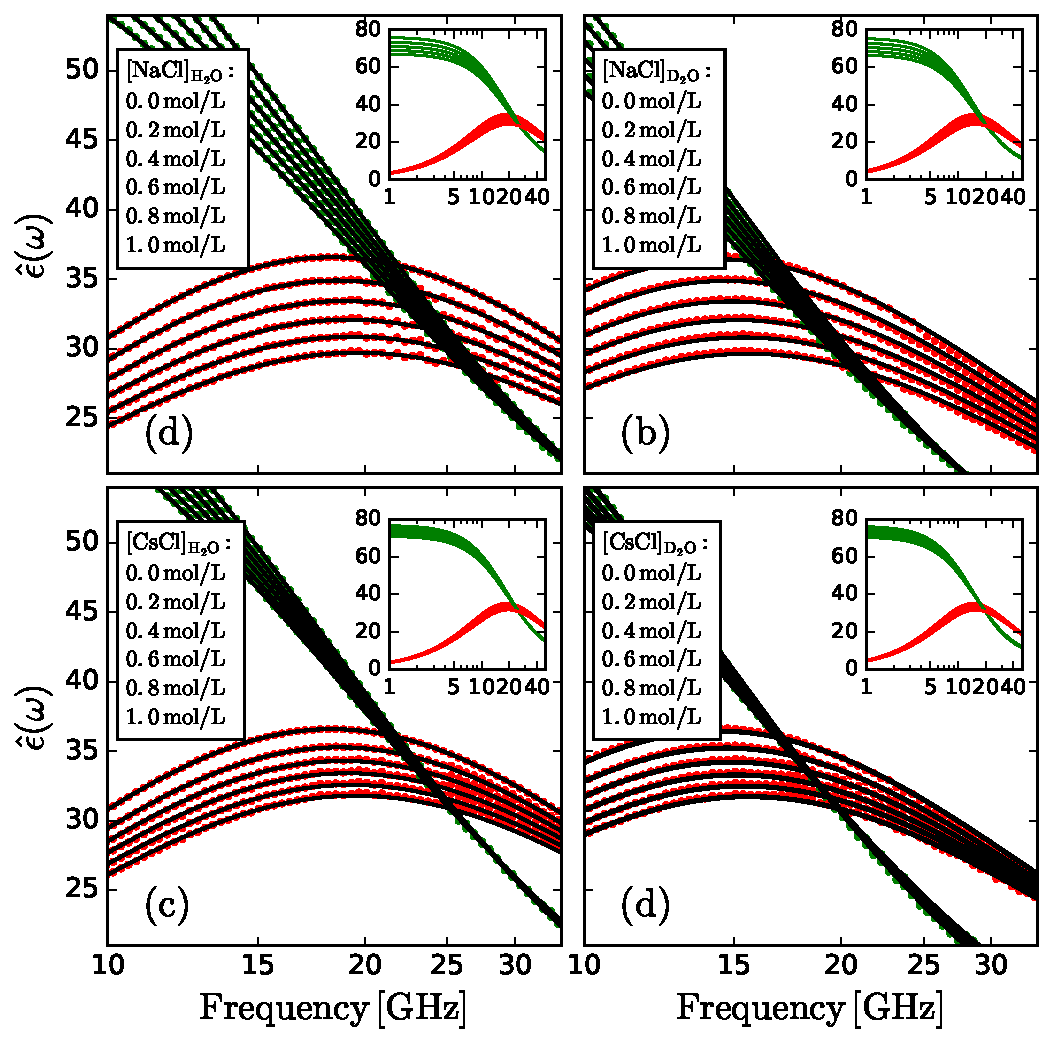
\includegraphics[width=0.9\figwidth]{chapters/Chapter4_PRL/Graphs/RawPermittivity_AllSolutions.pdf}
	\caption{Complex dielectric permittivity spectra of aqueous solutions of NaCl in H$_2$O (a), NaCl in D$_2$O (b), CsCl in H$_2$O (c) and CsCl in D$_2$O ranging from the neat solvent to 1.0 mol/L at 23$^o$C. The red and green dots indicate the data measured by DRS for the dielectric diffusion $\epsilon'(\omega)$ and dielectric losses $\epsilon''(\omega)$, respectively. The solid lines are fits to Eq.~\ref{epsilon}. All data is tabulated in the Appendix.}
	\label{fig1_Chap4}
\end{figure}
%\end{figure*}



Figure~\ref{fig1_Chap4} shows the complex permittivity of the investigated solutions, after subtraction of the ionic-conductivity contribution. Both the addition of NaCl and CsCl leads to a significant reduction of the dielectric response. 
The curves in Figure~\ref{fig1_Chap4} are the result of the least-squares fits, and Figure~\ref{fig2_Chap4}a shows the concentration-dependent conductivity $\sigma$ obtained from the fits. The values in H$_2$O agree well with previous results (see Appendix).\!\cite{Buchner1999,Bianchi1989} The conductivities of all the solutions are well described by the empirical function $\sigma (c) = D c - E c^{3/2}$, which has the same functional form as Kohlrausch's law that applies to dilute solutions. To correct the $A_\text{D}$ obtained from the fit for the trivial dilution effect, we define the concentration-dependent quantity
\begin{eqnarray}
A_\text{D,n}(c) = \frac{c_\text{w}(c)}{c_{\text{w},0}} A_{\text{D},0},
\label{eq4}
\end{eqnarray}
with $A_{\text{D},0}$ and $c_{\text{w},0}$ the amplitude of the Debye relaxation and the molecular concentration of undiluted neat water, and $c_\text{w}(c)$ is the water concentration of the electrolyte solution.
$A_\text{D,n}$ is the (hypothetical) dielectric strength if the only effect of ions in water would be a reduction in water concentration. The dilution-corrected depolarization
\begin{equation}
\Delta A_\text{D} = A_{\text{D,n}} - A_\text{D},
\end{equation}
is the depolarization caused by the interaction of the ions and the water. In the following, the term depolarization will refer to this dilution-corrected quantity $\Delta A_\text{D}$.





Figure~\ref{fig2_Chap4}b shows that the depolarization $\Delta A_\text{D}$ increases with concentration. In addition, there is a small but significant isotope effect: the depolarization is larger for D$_2$O than for H$_2$O solutions. This can be seen more clearly in Figure~\ref{fig3_Chap4}, where we present the isotope-difference $\Delta A_{\rm D}^{\rm H_2O}-\Delta A_{\rm D}^{\rm D_2O}$ as a function of concentration.  Dividing this difference by the value of $\Delta A_{\rm D}$ itself (Fig.~\ref{fig2_Chap4}b), we find that the isotope-effect is $\sim$1.5\% for NaCl and $\sim$3\% for CsCl solution.  The depolarization consists of a static and kinetic contribution:\!\cite{Hubbard1977,Hubbard1977a,Hubbard1979a,VanderZwan1982,VanderZwan1983a,Barthel1992} $\Delta A_{\rm D} = \Delta A_{\text{D,st.}} + \Delta A_{\text{D,kin.}}$ The dipole moments of H$_2$O and D$_2$O differ by only 0.06\%,\!\cite{Clough1973} which is negligible compared to the observed isotope effect, and to the uncertainty in our data. Hence, the static contributions to the depolarization can be assumed equal for H$_2$O and D$_2$O, so that 
\begin{equation}
\Delta A_{\rm D}^{\rm H_2O}-\Delta A_{\rm D}^{\rm D_2O} = \Delta A_{\rm D,kin.}^{\rm H_2O}-\Delta A_{\rm D,kin.}^{\rm D_2O}
\label{Skin} 
\end{equation}

The preceding result enables us to determine the kinetic depolarization independently from the static depolarization. In particular, we can directly compare the experimentally observed $\Delta A_{\rm D,kin.}^{\rm H_2O}-\Delta A_{\rm D,kin.}^{\rm D_2O}$ to theoretical predictions.  




%\begin{figure*}[ht]
\begin{figure}[t!]
	\centering
	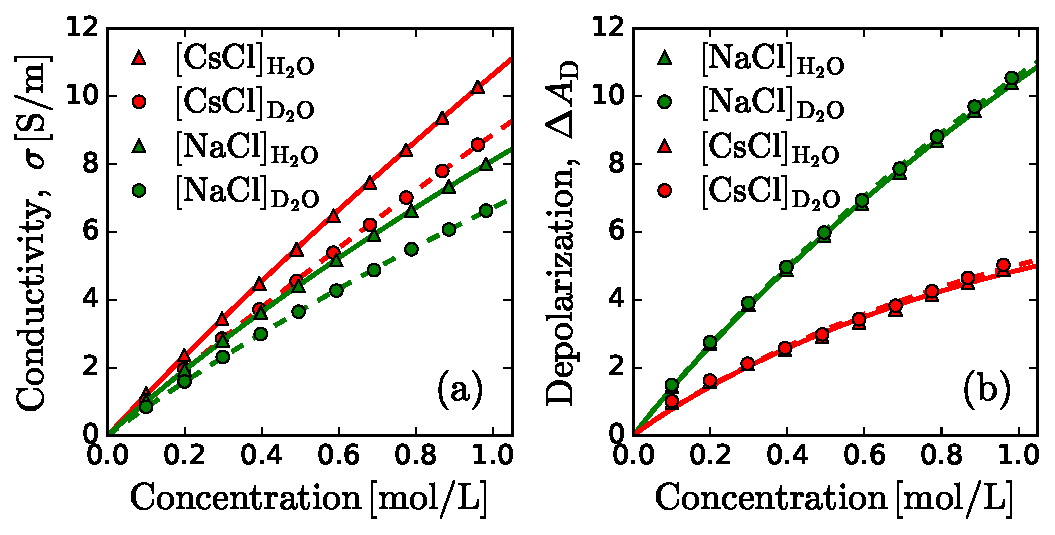
\includegraphics[width=0.85\figwidth]{chapters/Chapter4_PRL/Graphs/Conductivity_and_Depolarization.pdf}
	\caption{(a)~Conductivity $\sigma$ as a function of the salt concentration for four salt solutions. (b)~Depolarization as a function of concentration for the same solutions as in the left panel. The triangles and circles represent ions dissolved  in H$_2$O and D$_2$O, respectively; red and green refer to solutions with Na$^+$ and Cs$^+$ ions, respectively.}
	\label{fig2_Chap4}
\end{figure}
%\end{figure*}

\section{Determining the reduced cooperativity of water near ions}




The most commonly used model for kinetic depolarization is the continuum model derived by Hubbard and Onsager\!\cite{Hubbard1977,Hubbard1979a} (see Section \ref{SectionDepola}). In this model, the response of the water surrounding the moving ions is described as a continuum exhibiting the same Debye-relaxation behaviour as bulk neat water. Provided that the viscous frictional forces are much larger than 
the dielectric drag, the predicted kinetic depolarization is then given by
\begin{eqnarray}
\Delta A_{\text{D,kin.}}^{\rm HO} = p \sigma(c)  \left( \frac{ \tau_{\rm D} }{  \epsilon_0} \cdot \frac{\epsilon_s -\epsilon_{\infty}}{\epsilon_s }   \right),
\label{HOeq}
\end{eqnarray}
where $\sigma(c)$ is the concentration-dependent specific conductivity, $\tau_{\rm D}$ the Debye-relaxation time, and $p$ a factor which characterizes the tangential contact forces between the water molecules and ion surface, the limiting cases being perfect slip (no tangential force, $p = 2/3$), and perfect stick (infinite tangential force, $p=1$). This equation has no explicit dependence on the size of the ions. 
Since we measure all the parameters entering Eq.\ \ref{HOeq} for both H$_2$O and D$_2$O, we can directly test the validity of the Hubbard-Onsager model for the kinetic depolarization using Eq.~\ref{Skin}. The red lines in Figure~\ref{fig3_Chap4} are the theoretical predictions  for perfect slip (solid lines) and perfect stick (dashed lines). Clearly, the Hubbard-Onsager model predicts a much larger H$_2$O/D$_2$O difference in kinetic depolarization than is observed experimentally.

In a later, more rigorous theory for the kinetic depolarization, Hubbard, Colonomos and Wolynes describe the system as ionic spheres immersed in a solution of rotating dipoles, which are again assumed to exhibit Debye relaxation identical to that of bulk water. In this model the finite size of the solvent molecules is taken into account (as opposed to the earlier continuum model). They obtained an expression for the depolarization in which the radius of the ion occurs explicitly:\!\cite{Hubbard1979a} 
\begin{eqnarray}
\Delta A_{\text{D,kin.}}^{\rm HCW} = \frac{p \sigma(c) \tau_{\rm D}}{ \epsilon_0} \left[ \frac{N R_i}{e} \left\langle \frac{ \vec{\mu} \cdot \hat{r}}{r^2} \right\rangle \right], 
\label{HCWeq}
\end{eqnarray}
where $N$ is the number of water dipoles per volume unit, $R_i$ the ionic radius, $\mu$ the water molecule dipole moment, $r$ the distance between the water molecule and the ion and $e$ the ionic charge. In Ref.~\citenum{Hubbard1979a} the authors numerically evaluated the number in square brackets in Eq.~\ref{HCWeq}, in particular for Na$^+$, Cs$^+$ and Cl$^-$. 
The $\Delta A_{\text{D,kin.}}^{\text{H}_2\text{O}} - \Delta A_{\text{D,kin.}}^{\text{D}_2\text{O}}$ predicted by this theory is shown as the green lines in Figure~\ref{fig3_Chap4}, again for both limiting values of $p$. Again, the theory predicts a much larger difference in kinetic depolarization than is observed experimentally.


%\begin{figure*}[ht]
\begin{figure}[t!]
	\centering
	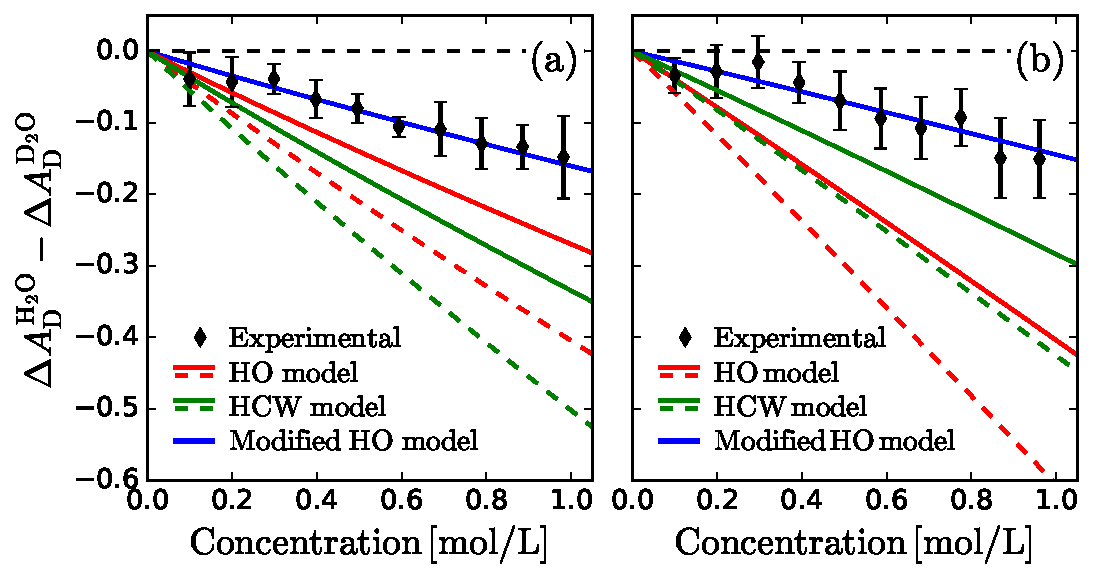
\includegraphics[width=0.85\figwidth]{chapters/Chapter4_PRL/Graphs/Onsager_Sodium_Caesium_EffectiveKirkwood_with_Fitting.pdf}
	\caption{(a)~Difference between the depolarization of NaCl in H$_2$O and the depolarization of NaCl in D$_2$O as a function of concentration. (b)~Difference between the depolarization of CsCl in H$_2$O and the depolarization of CsCl in D$_2$O as a function of concentration. The experimental results are represented by the diamonds. The solid lines represent calculations of the depolarization difference with different models for the kinetic depolarization using $p=2/3$ (solid lines) and $p=1$ (dashed lines). The solid blue line represents a fit to the data with the modified Hubbard-Onsager model of Eq.~\ref{eq:HOM}.}
	\label{fig3_Chap4}
\end{figure}
%\end{figure*}


The discrepancy between the theoretically predicted and experimentally observed kinetic depolarization can be explained if the water surrounding the ions exhibits a smaller dielectric response than bulk water. In neat water, the highly organized hydrogen-bond structure leads to highly cooperative reorientational motion of water molecules. As a consequence, the theory for the dielectric response of a liquid consisting of randomly moving dipoles (originally derived by Onsager\!\cite{Onsager1936a}) predicts a dielectric constant that is much smaller than observed. This is phenomenologically corrected in the Kirkwood-Fr\"ohlich equation:
\begin{equation}
\frac{(\epsilon_{\rm s}-\epsilon_\infty)(2\epsilon_{\rm s}+\epsilon_\infty)}
{\epsilon_{\rm s}(\epsilon_\infty+2)^2}=\frac{\rho \mu^2 g_\text{K}}{9 \epsilon_0 k_{\rm B}T} \qquad
\Rightarrow \qquad
\epsilon_{\rm s} \approx \frac{\rho \mu^2 g_\text{K}}{18 \epsilon_0 k_{\rm B} T}{(\epsilon_\infty + 2)^2},
\label{kirkwoodfroelich}
\end{equation}
where $\rho$ is the density of water molecules, $k_{\rm B}$ Boltzmann's constant, $\mu$ the molecular dipole moment, and $g_\text{K}$ the Kirkwood correlation factor  (see Section~\ref{KirkFrohSection}). The limit $g_\text{K}=1$ corresponds to completely uncorrelated motion of the molecules, and $g_\text{K}>1$ to correlated motion. For bulk liquid water, the experimentally determined value is $g_\text{K,bulk}= 2.7$. As can be seen in Eq.~\ref{kirkwoodfroelich}, the Kirkwood factor effectively scales up the dielectric response with respect to its theoretical value in the case of completely uncorrelated orientational motion.

The Hubbard-Onsager expression for the kinetic depolarization assumes that the dielectric response of water surrounding ions is the same as that of bulk water, i.e.\ that it has a Kirkwood factor of 2.7. However, ions tend to disrupt the hydrogen-bond structure of liquid water, and thus the reorientation of the water molecules surrounding the ions will be less correlated than that of the molecules in bulk water. To account for this effect, we modify the Hubbard-Onsager expression as follows:
\begin{equation}
%\Delta S_{\rm kin.}^{\rm eff.} = \left(\frac{g_{\rm ion}}{g_{\rm bulk}}\right) \Delta S_{\rm kin.}^{\rm HO}
\Delta A_{\text{D,kin.}}^{\rm HO,mod.} = \frac{p \sigma(c) \tau_{\rm D} }{ \epsilon_0 }\frac{g_\text{K,ion}}{g_\text{K,bulk}} \left[ \frac{\epsilon_s -\epsilon_{\infty}}{\epsilon_s } \right],
\label{eq:HOM}
\end{equation}
%\begin{figure*}[ht]
\begin{figure}[t!]
	\centering
	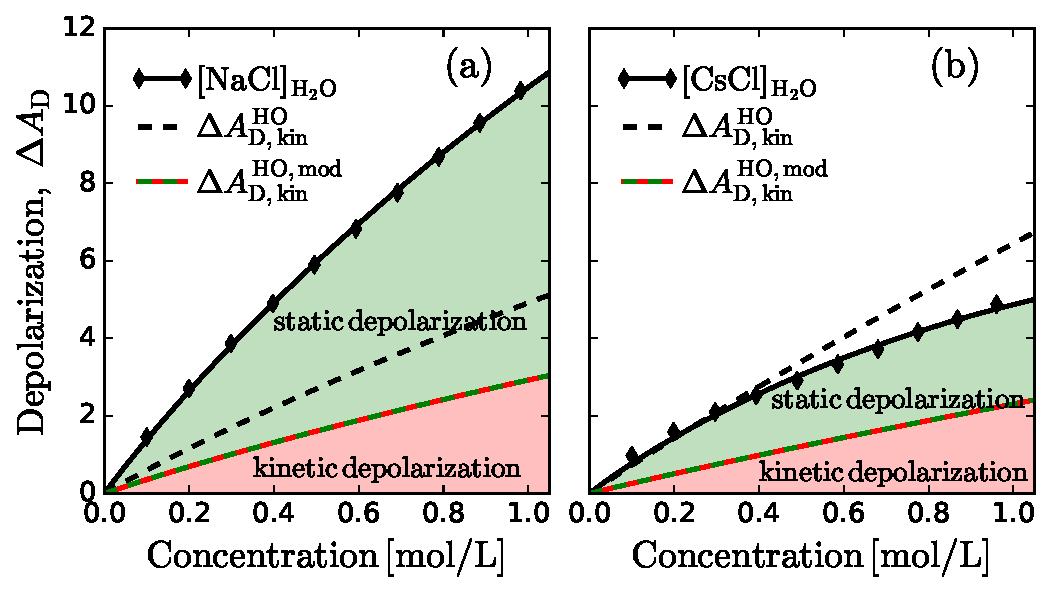
\includegraphics[width=0.85\figwidth]{chapters/Chapter4_PRL/Graphs/DepolarizationSeparation2.pdf}
	\caption{Experimentally observed total depolarization (corrected for dilution) of NaCl (a) and CsCl (b) in H$_2$O, and its decomposition into the static and the kinetic depolarization using the modified Onsager-Hubbard model~(Eq.\ \ref{eq:HOM}). The dashed black curve shows the kinetic depolarization predicted by the conventional Hubbard-Onsager equation. In the case of CsCl the conventional Hubbard-Onsager equation predicts a kinetic depolarization that is larger than the observed total depolarization, which would imply a negative static depolarization, and thus a negative hydration number.}
	\label{fig:HOM}
\end{figure}
%\end{figure*}
where we have introduced an effective Kirkwood factor $g_\text{K,ion}$ for the water surrounding the ions. The value of $g_\text{K,ion}$ can be determined by fitting the above equation to the experimental data (and using the known value of $g_\text{K,bulk}$), see the blue lines in Figure~\ref{fig3_Chap4}. We find $g_\text{K,ion}$ values of 1.6$\pm$0.1 and 1.0$\pm$0.2 for Na$^+$ and Cs$^+$, respectively. The smaller value for Cs$^+$ compared to Na$^+$ is due to a stronger propensity to break up the hydrogen-bond structure of water. This result is in line with previous investigations of the relation between water structure and ionic mobility,\!\cite{Kay1966,Hertz1974,Hertz1976,Harris1978} which showed faster ionic diffusion in less structured hydrogen-bond environments. At high concentrations, the Hubbard-Onsager theory will also overestimate the amplitude of the kinetic depolarization because this theory does not include the Debye screening of the potential of the moving charge due to the dynamic repositioning of the other ions in the medium. We will not consider this effect here, but we hope that our experiments will stimulate further experimental and theoretical work in this direction.






Using the modified Hubbard-Onsager equation, we can now decompose the observed (dilution-corrected) depolarization into its static and kinetic contributions in a well-defined manner. The result is shown in Figure~\ref{fig:HOM}, which also displays the kinetic depolarization predicted by the conventional Hubbard-Onsager equation (Eq.~\ref{HOeq}). Note that by subtracting the latter from the total depolarization one obtains a negative static depolarization for CsCl, which is not physically meaningful. Using the modified Hubbard-Onsager equation we obtain a positive (physically meaningful) static depolarization.




\section{Discussion and conclusion}


From the amplitude of the static depolarization we can directly estimate the number of water molecules that are rotationally immobilized per ion, i.e.\ the hydration number.\!\cite{Barthel1992} We obtain hydration numbers of 8.1$\pm$0.9 for Na$^+$ and 3.1$\pm$1.0 for Cs$^+$. These numbers agree well with previous estimates obtained using more indirect measurements.\!\cite{Richens1997} Both for Na$^+$ and Cs$^+$ the hydration number (the number of rotationally immobilized water molecules) is different from the coordination number (the number of water molecules that in the first solvation shell: 6 and 8 for Na$^+$ and Cs$^+$ respectively).\!\cite{Ohtaki1993,White2000,Varma2006,Mason2006,Rowley2012} This difference is a general phenomenon\!\cite{Barthel1992} which illustrates the importance of experimentally determining the hydration number.

To conclude, the observed isotope effect in the depolarization of ionic solutions indicates that water molecules surrounding ions reorient in a much less cooperative manner than in neat bulk water, with Kirkwood factors close to unity. Based on our observations we propose a modified Hubbard-Onsager equation that takes the locally reduced Kirkwoord factor into account, and that makes it possible to analyze the depolarization of ionic solutions in an unambiguous manner.  This modified Hubbard-Onsager equation provides meaningful hydration numbers, which the conventional Hubbard-Onsager equation fails to do (in some cases even leading to unphysical results) because this expression overestimates the collective nature of water reorientation near ions. Our results thus provide new insights into the effect of ions on water cooperativity. The approach presented here enables a reliable determination of hydration numbers, which is of broad physical relevance, since hydration numbers are widely used to quantify the physical and chemical properties of aqueous solutions.


